% !TeX root = ../main.tex

\chapter{实现}

这一章将描述我们提出的上界验证算法的具体实现。我们的实现主要是基于\texttt{Ultimate}这一模块化的程序分析套件,并结合C语言的标注语言ACSL的输入格式,以及程序验证中间语言Boogie的已有技术。本章先简要介绍相关的工具,然后对算法的实现进行描述。

\section{\texttt{Ultimate} 程序分析套件概述}

\texttt{Ultimate}程序分析套件\cite{heizmann_software_2013, heizmann_termination_2014,chen_advanced_2018}是由弗莱堡大学的学者和研究人员开发和维护的一套工具,由Java编写。它也可以被认为是一个用于开发程序分析工具的框架,采用模块化的插件(plugin)系统,由一个个的插件实现和提供不同的程序分析方法。这些插件能实现从源代码解析、程序表示的转化到静态分析的一系列功能,而通过将这些插件相互组合为工具链(toolchain),可以完成非常复杂的程序分析任务。作为程序验证工具而言,\texttt{Ultimate}涵盖了安全属性检查\cite{heizmann_software_2013}、终止性分析\cite{heizmann_termination_2014}、模型检测、并发程序验证等主要领域的需求,实现了大量的主流算法。

\texttt{Ultimate}可以接受多种语言的程序,但最主要的源语言是C语言。我们可以编制一个工具链,使用\texttt{Ultimate}验证C语言程序的安全属性。图\ref{fig:ultimate-example}比较直观地展示了主要插件之间的关系。

\tikzstyle{process} = [rectangle, minimum width=3cm, minimum height=1cm, text centered, draw=black]

\begin{figure}
    \centering
    \begin{tikzpicture}
        \node (pro1) [process] {ACSL标注的C语言文件};
        \node (pro2) [process, below of=pro1] {C抽象语法树};
        \node (pro3) [process, below of=pro2] {Boogie中间表示};
        \node (pro4) [process, below of=pro3] {控制流图};
        \node (pro5) [process, below of=pro4] {验证结果或反例};
        \draw (pro1) -- node [left] {CDTParser} (pro2);
        \draw (pro2) -- node [left] {CACSL2BoogieTranslator} (pro3);
        \draw (pro3) -- node [left] {RCFGBuilder} (pro4);
        \draw (pro4) -- node [left] {TraceAbstraction} (pro5);
    \end{tikzpicture}
    \caption{\texttt{Ultimate}框架中,进行C语言程序安全属性检查时的工具链中各插件的关系,以及过程中的中间表示}
    \label{fig:ultimate-example}
\end{figure}

\texttt{Ultimate}会首先对C语言进行语法解析(插件CDTParser),得到抽象语法树,随后通过翻译过程,将其转换为Boogie这一中间表示(插件CACSL2BoogieTranslator)。在将Boogie程序转换为等价的CFG后(插件RCFGBuilder),最终进行以路径抽象(插件TraceAbstraction)为基础的安全属性检查过程\cite{heizmann_traces_2015}。

其中,Boogie\cite{leino_this_2016}是由微软提出的一种验证中间语言(intermediate verification language),类似于一般的IR,它的作用是简化高级语言验证器的开发。开发者可以实现从高级语言及其规范到Boogie的翻译,由Boogie求解器完成后续的验证。在此不赘述Boogie的语法,只给出以下代码\ref{listing:chap4-boogie-example}中的程序作为例子,从中可以看出,Boogie作为一门语言,在保留一般的命令式程序的框架的基础下保持简洁,删减了高级语言面向用户的若干特性。另外,Boogie中采用断言语句\textbf{assert} $\phi$来指定程序中的错误状态,这和\textbf{Imp}中使用独立的错误位置来代表安全属性的做法类似但稍有不同,不过这两种表示之间的对应关系是直观的。

\begin{listing}[ht]
\begin{minted}
[
frame=lines,
framesep=2mm,
baselinestretch=1,
fontsize=\footnotesize,
linenos
]{text}
procedure main()
{
  var n, p: int;

  assume p != 0;
  while (n >= 0) {
    assert(p != 0);
    if (n == 0) {
      p := 0;
    }
    n := n - 1;
  } 
}

\end{minted}
\caption{在Boogie语言中表示的简单函数以及对其的规范}
\label{listing:chap4-boogie-example}
\end{listing}

为了在C语言中表示对程序行为的规范,\texttt{Ultimate}允许输入程序在ANSI C的基础上使用ACSL进行标注。ACSL全称ANSI/ISO C Specification Language,是对C语言程序的行为进行规范的一种DSL,最早用于Frama-C\cite{kirchner_frama-c_2015}C语言程序分析套件中。ACSL可以表达丰富的规范,包括一般的行为正确性,以及和C语言中涉及的一些低级的机器细节相关的规范。代码\ref{listing:chap4-acsl-example}中的程序是一个用ACSL进行标注后的简单程序,其中,ACSL标注存在于C语言的注释之中,它既可以出现在函数定义之前,也可以出现在循环结构之前。

\begin{listing}

\begin{minted}
[
frame=lines,
framesep=2mm,
baselinestretch=1,
fontsize=\footnotesize,
linenos
]
{c}
/*@
  requires \valid(a+(0..n-1));

  assigns  a[0..n-1];

  ensures
  \forall integer i;
    0 <= i < n ==> a[i] == 0;
*/
void set_to_0(int* a, int n){
  int i;

  /*@
    loop invariant 0 <= i <= n;
    loop invariant
    \forall integer j;
      0 <= j < i ==> a[j] == 0;
    loop assigns i, a[0..n-1];
    loop variant n-i;
  */
  for(i = 0; i < n; ++i)
    a[i] = 0;
}
\end{minted}

\caption{使用ACSL标注的C语言程序示例}
\label{listing:chap4-acsl-example}
\end{listing}

\section{上界算法的实现}

\subsection{对ACSL的扩展}

ACSL中并没有能表达上界的语法结构,为了让用户能方便地在源文件中指定循环上界,我们对ACSL的语法进行了扩展,引入了如下的循环上界语句:

\[
\mathbf{loop} \, \{name\} \,\mathbf{bound} \,  \phi \, \{\mathbf{scope} \, nested\}
\]

循环上界语句和不变式语句一样,只能出现在循环之前,并对此循环的性质进行说明。其中,$\phi$是上界的符号表达式;\textit{name}是一个标识符,相当于给当前循环打上标签或起的名称;\textit{nested}也是一个标识符,它是当前循环所在的某个嵌套循环的名称,代表的是当前循环的上界的作用域。后者的存在是为了解决实际程序中可能出现的多层嵌套的情况。\textit{name}和\textit{nested}都是可选的。如果不指定\textit{nested},则对应于定义\ref{def:chap3-proof-structure}中的“global”作用域,即指定的是全局意义下的循环上界。例如,代码\ref{listing:chap4-acsl-bound}中的程序中有嵌套循环,我们分别用ACSL对其进行了标注。

\begin{listing}

\begin{minted}
[
frame=lines,
framesep=2mm,
baselinestretch=1,
fontsize=\footnotesize,
linenos
]{c}

void while2(int a, int b, int c) {
  a = b;
  //@ loop l1 bound max(b, 0);
  while (a >= 1) {
    c = b;
    //@ loop l2 bound max(b, 1) scope l1;
    while (1) {
      if (c >= 1) {
        c = c - 1;
      }
      else if (0 >= c) {
        a = a - 1;
        break;
      }
      else
        return;
    }
  }
}

\end{minted}
\caption{一个使用ACSL扩展对上界进行标注的C语言程序}
\label{listing:chap4-acsl-bound}
\end{listing}

我们修改了\texttt{Ultimate}框架的前端部分以支持新的语法,并加入了检测步骤确保语句中作用域的嵌套是合法的,即不会形成环路。显然,如果程序中每个自然循环都进行了标注,并通过检查,所得到的标注语句构成了一个证明结构。

\subsection{扩展语法的翻译}

我们沿着上一章证明结构的验证思路,实现了从C语言到Boogie的翻译过程的修改。假设每个自然循环$L$都有唯一的上界标注,这意味着一个上界表达式$\phi_L$,以及可选的名称$N_L$和作用域标识$S_L$。将ACSL标注翻译为Boogie的过程和C语言到Boogie的翻译过程紧密相连,我们假设\textbf{Translate}是C语言的翻译过程,给定一个C语言函数它返回对应的Boogie函数。

ACSL扩展部分的翻译例程如算法\ref{alg:chap4-c-to-boogie}所示。我们将翻译分为两个步骤:首先对循环进行后序遍历,将每个循环需要额外添加到作用域(或函数)入口处以及循环体入口处的语句分别记录在变量Reset(或Global)和Body中。接着,我们调用\textbf{Translate}完成函数的翻译,并在得到的新函数$P'$中插入上述语句。

\begin{algorithm}
    \begin{algorithmic}
        \REQUIRE C语言函数定义$P$
        \ENSURE Boogie函数定义$P'$
        \STATE Global $\leftarrow \{\}$ \COMMENT Global是语句的集合
        \STATE Reset $\leftarrow \{\}$ \COMMENT Reset是从循环到语句的映射
        \STATE Body $\leftarrow \{\}$ \COMMENT Body是从循环到语句的映射
        
        \STATE iter $\leftarrow$ $P$中所有自然循环的后序遍历迭代器
        \WHILE{$iter.hasNext$}
        
            \STATE L $\leftarrow$ $iter.next$
            
            \IF{$S_L = "global"$}
                \STATE $Global.add(i_L = \phi_L)$
            \ELSE
                \STATE $Reset(Name2Loop(S_L)).add(i_L = \phi_L)$
            \ENDIF
            \STATE $Body(L).add(i_L = i_L - 1; assert(i_L \geq 0))$
            \STATE $Body(L).add(Reset(L))$
        \ENDWHILE
        
        \STATE 忽略$P$中上界标注,调用\textbf{Translate}将$P$翻译为Boogie函数$P'$
        \STATE 为$P$中所有自然循环$L$在$P'$中声明整型变量$i_L$
        \FORALL{自然循环$L \in P$}
            \STATE 将$Body(L)$加到$P'$中$L$对应的循环头之后
        \ENDFOR
        \STATE 将Global中的语句加到$P'$初始位置之后
        \RETURN $P'$
    \end{algorithmic}
    \caption{带ACSL上界标注的C语言函数的翻译流程}
    \label{alg:chap4-c-to-boogie}
\end{algorithm}
        
以代码\ref{listing:chap4-acsl-bound}中的C语言函数为例,翻译后得到的Boogie函数如代码\ref{listing:chap4-acsl-bound-boogie}所示。

\begin{listing}
\caption{翻译代码\ref{listing:chap4-acsl-bound}得到的Boogie程序}
\label{listing:chap4-acsl-bound-boogie}
\begin{minted}
[
frame=lines,
framesep=2mm,
baselinestretch=1,
fontsize=\footnotesize,
linenos
]{text}
implementation while2(#in~a : int, #in~b : int, #in~c : int) 
    returns ()
{
    // 省略变量声明部分...
    ~a := #in~a;
    ~b := #in~b;
    ~c := #in~c;
    if (~b > 0) {
        #t~ite0 := ~b;
    } else {
        #t~ite0 := 0;
    }
    #bound~1 := #t~ite0;
    ~a := ~b;
    while (true)
    {
      Loop~0:
        if (!(~a >= 1)) {
            break;
        }
        #bound~1 := #bound~1 - 1;
        assert #bound~1 >= 0;
        if (~b > 1) {
            #t~ite1 := ~b;
        } else {
            #t~ite1 := 1;
        }
        #bound~3 := #t~ite1;
        ~c := ~b;
        while (true)
        {
          Loop~2:
            if (false) {
                break;
            }
            #bound~3 := #bound~3 - 1;
            assert #bound~3 >= 0;
            if (~c >= 1) {
                ~c := ~c - 1;
            } else if (0 >= ~c) {
                ~a := ~a - 1;
                break;
            }
        }
    }
}
\end{minted}
\end{listing}

\subsection{验证失败时的反例}

我们采用\texttt{Ultimate}的安全属性检查器对得到的Boogie程序进行验证。在我们的形式化中,安全属性表述为“某些错误位置永远不会被访问”,因此,如果一条安全属性被违反,必然可以找到程序的有限长的执行到达错误位置,这就是此安全属性在程序中的反例(counterexample)。

给出反例可以让用户确定一组导致错误的输入参数值,并且沿着错误路径,理解程序为何会产生非预期的行为,帮助修改程序的实现。因此,验证工具应该尽量返回反例。

由于我们采用了将问题完全归约到安全属性检查的方法,安全属性检查器所返回的反例对于上界为何不成立也有着指导意义。尤其是,它给出了一组输入参数值(即初始状态$s_0$),使得以此组参数的值为输入时,程序的上界超过$s_0(\phi)$\footnote{因为程序中有非确定赋值语句\textbf{havoc},所以同样的参数可能有不同的执行路径。更准确的说法是存在一个以$s_0$为初始状态的执行,使得其上界超过$s_0(\phi)$。}。

如对于上述代码\ref{listing:chap4-acsl-bound}中的示例程序,我们的实现给出了否定的结果,并返回了一个反例,其中包括输入参数$b=1$。我们将其带入两个循环上界的表达式,分别得到外层和内层循环的上界都是1,但实际的执行中,外层循环被迭代1次,而每次迭代中,内层循环被迭代2次。由此可见内层循环的上界是错误的。实际上,因为这里有两个循环,故调整后的程序中有两个错误位置,而对于安全属性检查而言,只需有一个位置可达即可判定为属性不成立,故反例是从初始位置到某个可达错误位置的路径,这有助于帮助用户快速定位是哪一个循环上界发生了错误。

\section{实验与测试}

我们在\texttt{Ultimate}的ACSL语法解析和C到Boogie的翻译两个插件中实现了关于上界的规范的识别和验证,并将它嵌入到了\texttt{Ultimate}进行安全属性检查的工具链中,从而形成了一个可独立执行的工具。在这一节中,我们简要介绍对它的测试结果。

\subsection{测试集的选取与处理}

在引言中,我们以\texttt{Loopus}为例说明了自动上界生成工具的结构可能存在错误。因此,\texttt{Loopus}的测试集比较适合对本工具的验证效果,尤其是证伪的能力进行测试。\texttt{Loopus}的测试集是从\cite{brockschmidt_alternating_2014}中修改的,主要是C语言的各式算法,总共包含658个C语言程序。

我们对这些程序进行了筛选。首先是去除含有抽象数据结构、使用堆内存以及某些C语言扩展语法的文件;其次,我们分析程序中的循环结构的数量,去除了不含循环的程序(主要是从其他语言\footnote{\texttt{Loopus}的测试集中有很多来自T2这一工具,而T2的输入格式是类似于自动机的变迁系统,翻译为C语言后由一系列\textit{goto}语句组成}经由翻译得到的C语言程序);随后我们分析了\texttt{Loopus}给出的上界表达式,删除了那些无法用输入参数表示的表达式所在的测例。最终,我们得到了由152个C语言程序组成的测试集,大部分程序比较短小,它们的平均代码行数为22行。

\subsection{测试结果}

\texttt{Loopus}对这152个程序都给出了一个合法的上界。由于\texttt{Loopus}给出的上界是整个程序的上界,我们采取手动的方法将它们以ACSL标注到了程序中。表\ref{tab:chap4-result}给出了本文的工具在这些程序上得到的结果,工具是在4线程Intel\textregistered{} Core\texttrademark{} i7-7500U CPU @ 2.70GHz CPU上运行的,时间限制设置为1200秒,内存限制为8G。

\begin{table}[t]
  \centering
  \caption{本文工具在测试集上的运行结果}
  \begin{tabular}{lll}
    \toprule
    结果  & 数量 & 说明                        \\
    \midrule
    correct   & 12 & 给定的上界被证明是正确的 \\
    incorrect   & 122 & 给定的上界被证伪                   \\
    timeout  & 10   & 工具在1200秒内未能给出结果 \\
    unknown & 8 & 工具无法验证上界的正确性 \\
    \bottomrule
  \end{tabular}
  \label{tab:chap4-result}
\end{table} 

从表\ref{tab:chap4-result}中的结果可以看出,我们的工具能验证绝大部分的测例,而其中80\%的上界都是错误的。人工对部分被证伪的程序进行复杂度分析得到的结果确证了这一结论,这说明\texttt{Loopus}在其测试集上给出的结果大多数都是不正确的。考虑到\texttt{Loopus}采用的算法在理论上是可靠的\cite{sinn_simple_2014},这应是源于其工具在实现过程中出现的编码层面的偏差。此外,这一结果进一步表明了进行上界验证的必要性,我们需要填补自动上界生成工具只能生成,无法验证的空白。

我们进一步分析了验证失败的情况。上表中,结果为unknown的情况下C语言程序均被正确地翻译到了Boogie中间表示,但是\texttt{Ultimate}的安全属性检查器无法验证变换后的程序。正如在第\ref{section:chap2-safety-check}节中指出的,安全属性检查本身也是不可判定的问题,所以必然存在无法求解的情况。对此8个程序进行考察发现,其控制流基本上都比较复杂,部分程序中存在非线性的赋值,而目前的安全属性检查方法对线性程序和控制流简单的程序的支持较好,对复杂程序和非线性程序的支持不足。超时的测例类似,基本上也可以归因于程序的非简单结构。

虽然存在无法求解的情况,除去超时的测例,本文的工具进行求解的效率普遍较高,平均用时为1.37秒,最长用时67.1秒。图\ref{fig:chap4-performance}展示了各测例的用时,其中坐标为对数坐标。从中可以看出,对绝大部分程序进行验证所需的时间在3秒以内。这说明本文的工具可以较为高效地进行上界的验证。

\begin{sidewaysfigure}[]
    \centering
    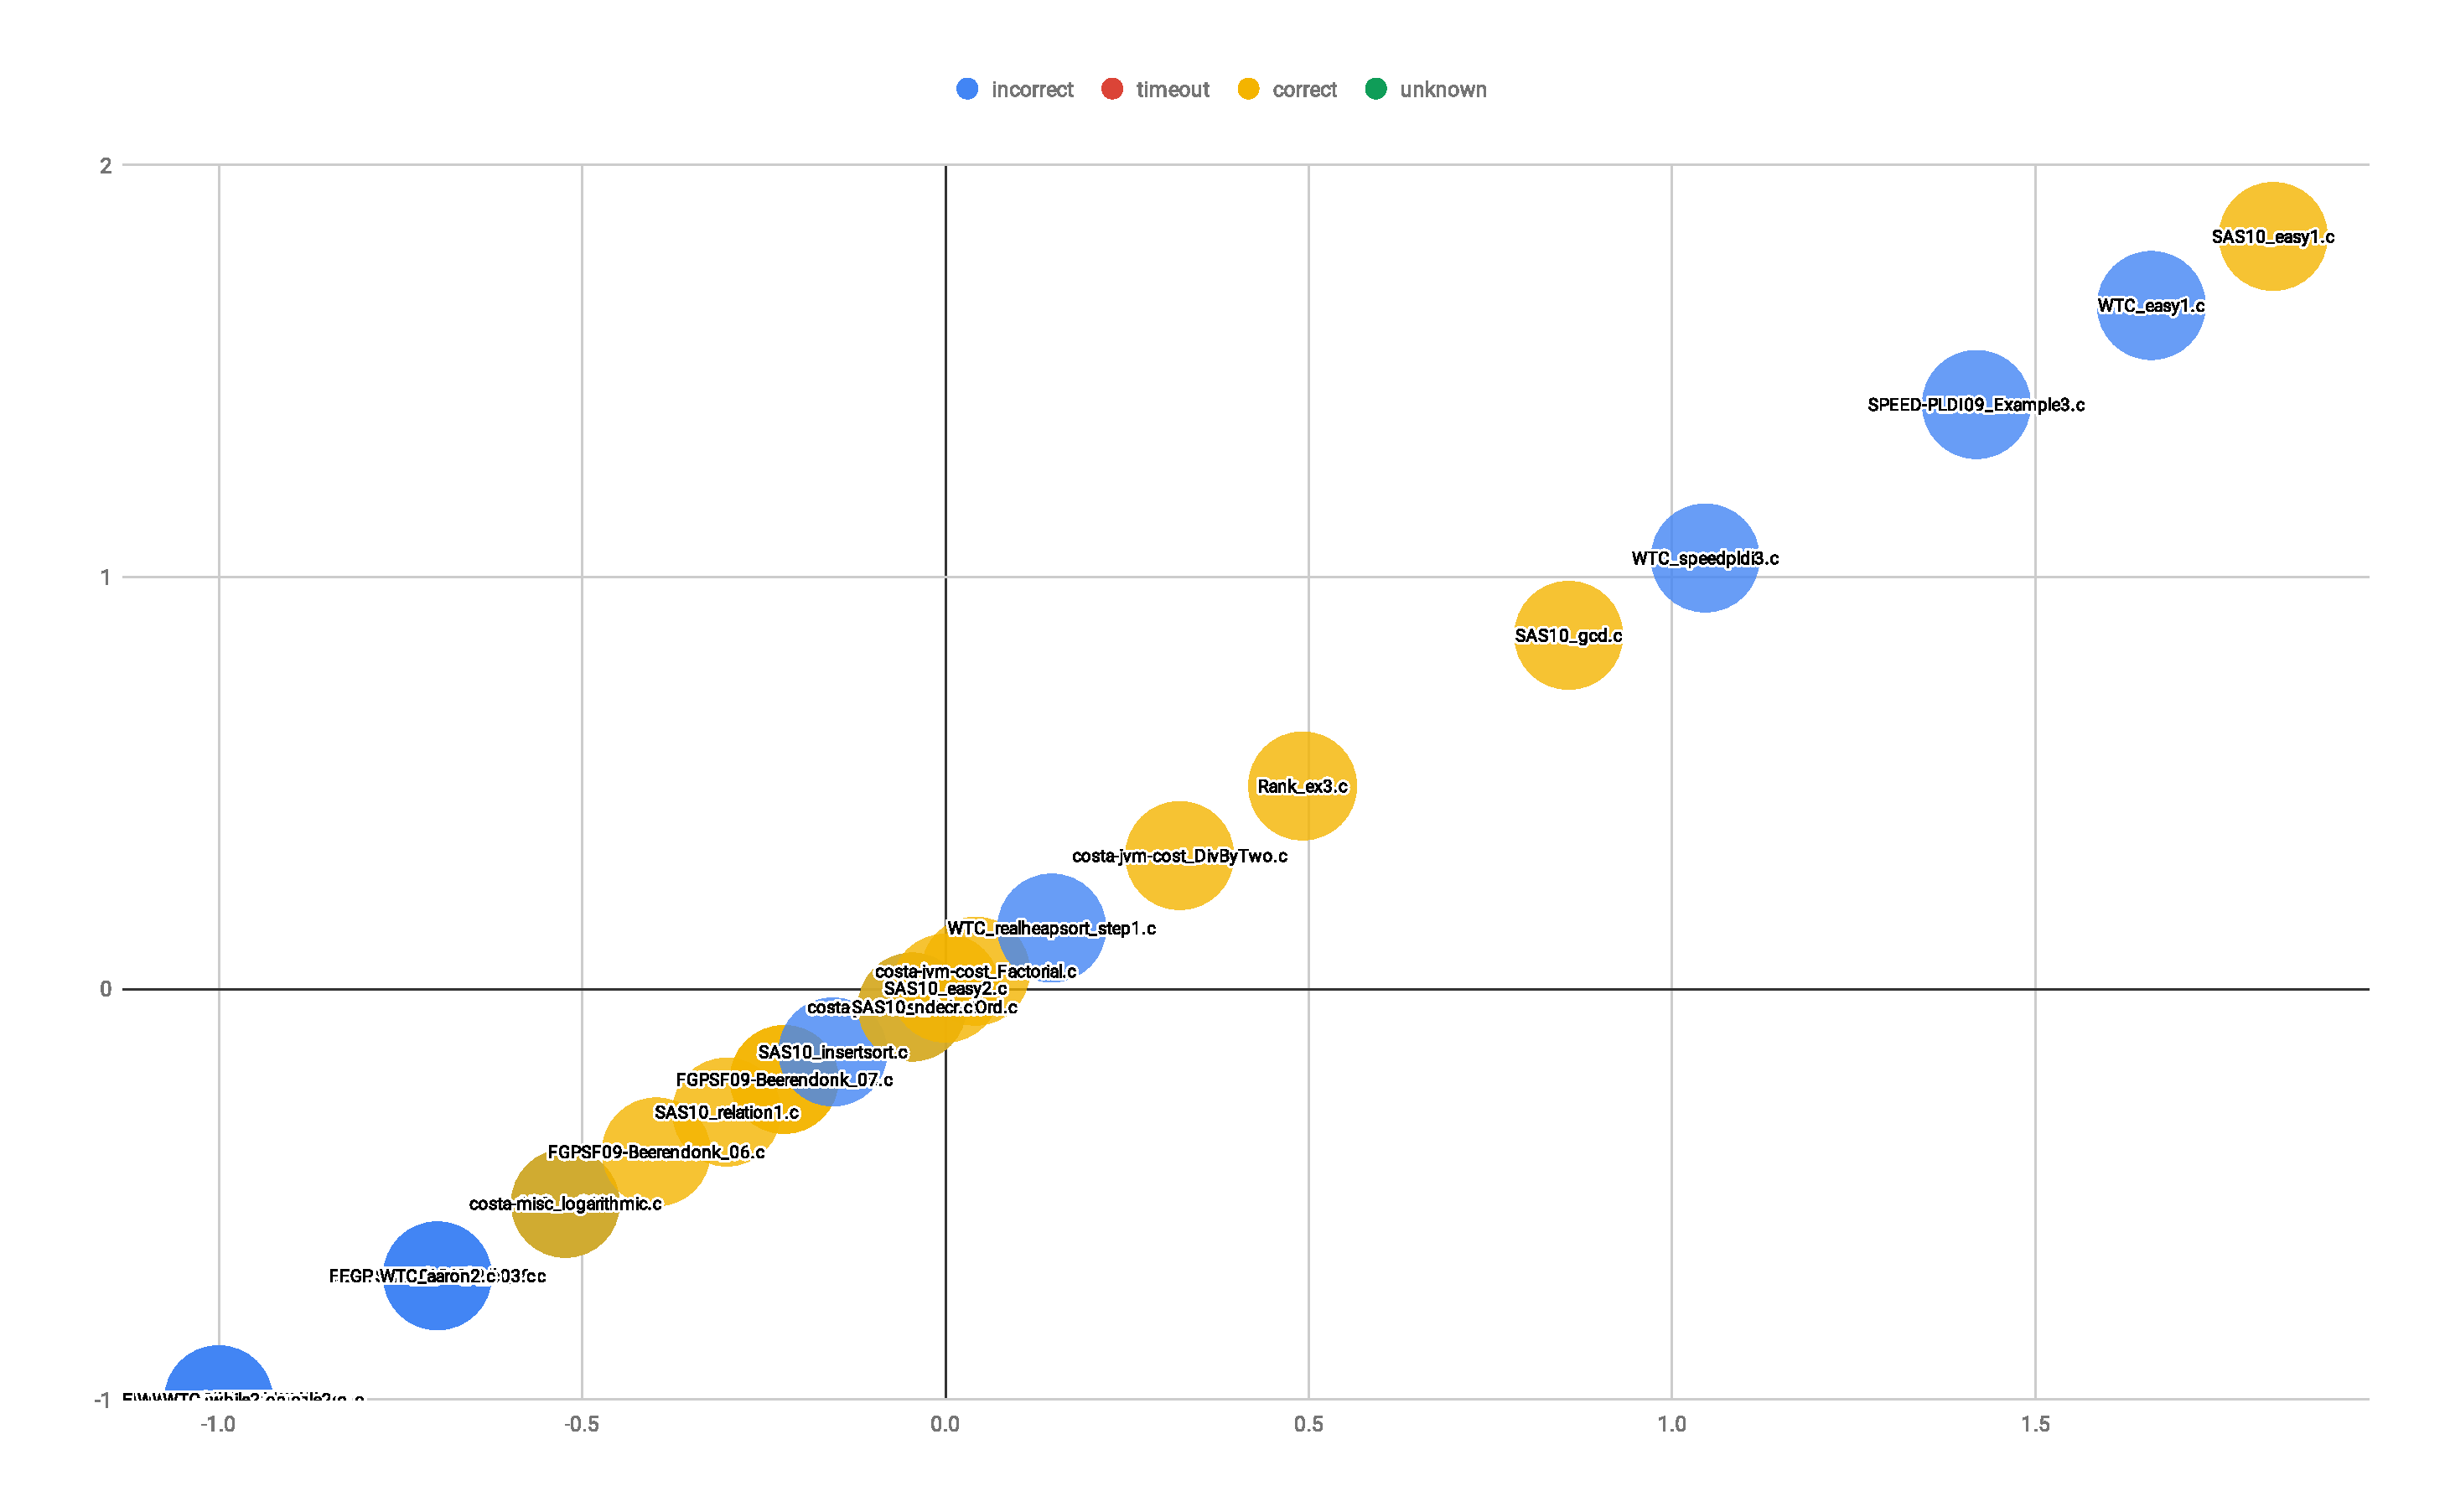
\includegraphics[width=\columnwidth]{chart.pdf}
    \caption{验证成功的测例用时(对数坐标)}
    \label{fig:chap4-performance}
\end{sidewaysfigure}

% 由于Loopus给出的上界中正确的部分较少,我们用人工的方式考察了上表中结果为错误的测例。对于其中行数较少,结构不太复杂的程序,我们对其进行复杂度分析,给出一个新的上界。我们最终得到了\todo{number}个程序的上界,比同样将它们用ACSL进行了标注。我们的工具能够顺利地验证所有这些程序的上界,说明算法对错误和正确的上界同样有效。